\documentclass{cumcmthesis}
% \documentclass[withoutpreface,bwprint]{cumcmthesis} %去掉封面与编号页,电子版提交的时候使用。


\usepackage[framemethod=TikZ]{mdframed}
\usepackage{url}   % 网页链接
\usepackage{subcaption} % 子标题
\title{全国大学生数学建模竞赛}
\tihao{A}
\baominghao{4321}
\schoolname{天津大学}
\membera{ 谢远峰}
\memberb{ 元祥渊}
\memberc{ 陈柯亘}
\supervisor{ 王宏}
\yearinput{2021}
\monthinput{09}
\dayinput{15}

\begin{document}

\maketitle
\begin{abstract}
    % cumcmthesis 是为全国大学生数学建模竞赛编写的\LaTeX{}模板, 旨在让大家专注于 论文的内容写作, 而不用花费过多精力在格式的定制和调整上. 本手册是相应的参考, 其 中提供了一些环境和命令可以让模板的使用更为方便. 同时需要注意, 使用者需要有一 定的 \LaTeX{} 的使用经验, 至少要会使用常用宏包的一些功能, 比如参考文献,数学公式,图片使用,列表环境等等. 例子文件参看 \texttt{example.tex}.
    目的:本篇文章基于传染病SEIRD模型研究美国阿肯色州COVID-19发展趋势,使用python工具建立传染病模型,仿真揭示美国阿肯色州从2020年3月6日到2021年3月6日的疫情情况。

    方法:研究选取covid\_tracking.csv数据集,通过python分析数据,使用微分方程传播模型求解。最终得出仿真模拟预测结果,与实际值进行比较。

    结论:我们针对美国阿肯色州的病毒传播情况进行建模并对比观察。我们认为严格的疫情防控和控制移动范围、控制聚集等活动对COVID-19的传染起到了良性作用,为了减小感染病毒可能性,减少大型集会、减少跨区域移动对防控病毒的传播起到有效作用。就疫苗接种而言,各州从有效率角度考虑,需尽可能多选择辉瑞和Moderna疫苗,并减少聚集。


    \keywords{COVID-19 \quad Python\quad   SEIRD模型}
\end{abstract}


\tableofcontents

\clearpage
\section{数学模型的建立和分析}
\subsection{假设与符号说明}
对于该数学问题我们有以下几点假设:
\begin{itemize}
    \item 疫情统计数据是可靠的
    \item 病人处于潜伏期时无传染性,潜伏者均会转变为感染者,感染后康复不会再被感染
    \item 选定地区迁入和迁出人口大致相等,不考虑出生和自然死亡,即总人口基本不变
    \item 人群均匀混合。任何感染者以概率$\alpha$ 接触其它易感者,概率用总体均值替代
    \item 病毒处于稳态,未发生变异,疾病的传播率固定
    \item 假设人群中只能通过感染新冠病毒进行患病
    \item 死亡人群不再具有感染性,从感染人群中剔除
    \item S:易感人群;E:传染人群;I:感染人群;D:死亡人群;R:康复人群
    \item $\beta$:传染率;$\sigma$:发病率;$\mu$:死亡率;$\gamma$:康复率
\end{itemize}

\subsection{分析问题}
2020年威胁人类健康的新型冠状病毒传染率高、无特定易感人群、有一定致死率,已经在全球范围传播。美国政府在初期不作为,导致了国内人民遭受了大面积的疫情袭击。我们选取了阿肯色州(Arkansas)作为目标,对该地区的疫情情况进行建模和分析。考虑到新冠肺炎具有明显的潜伏期以及高于一般传染病的致死率,基于基本的SIR模型,调整采用更适用于恶性传染病的SEIRD模型;并在完成模型构建的基础上,与已有的疫情统计数据相结合,对阿肯色州地区的疫情作出分析。
\subsection{基础模型}
\clearpage
\subsection{建立数学模型}
新冠肺炎没有特定的易感人群,但是可以确定的是免疫力低下的人群和接触人员更多的人群更容易患病,因此我们将这一部分人设置为S,即该模型中的易感人群;使用E表示被病毒传染的人群,使用I来表示感染人群,潜伏人群E经过一定的潜伏期后均会变成感染人群S。D表示死亡人群,R表示康复人群。$\beta$是传染率, 反映病毒传播的快慢;$\sigma$为发病率,表示潜伏者转变成感染者的概率,它的倒数是潜伏期天数;$\mu$为死亡率,表示的是感染者因新冠肺炎死亡的概率;$\gamma$为康复率, 表示感染者恢复健康的概率。

\vspace*{0.2cm}
\begin{enumerate}
    \setlength{\itemsep}{2pt}
          \setlength{\parsep}{2pt}
          \setlength{\parskip}{2pt}
    \item $\frac{dS}{dt}= -\frac{\beta SI}{N}$:易感者随时间变化
    \item $\frac{dE}{dt}=\frac{\beta SI}{N}-\sigma E$:传染者(潜伏期)E随时间t变化
    \item $\frac{dI}{dt}=\sigma E-\gamma I- \mu I$:感染者随时间t的变化
    \item 感染者随时间发展转变为两部分,死亡者D/康复者R
    \item $\frac{dR}{dt}=\gamma I$:康复者随时间t的变化
    \item $\frac{dD}{dt}=\mu I$:死亡者随时间t的变化
    \item N=S+E+I+R+D:模型涉及的人口总和
\end{enumerate}

其中$\beta$参数与系数R0成正比。R0通常由传染病学家分析疫情特定情况得出,表示的是疾病的传染性,R0决定了一个感染者可以将疾病传染给多少个人。若R0<1,则传染有希望停止;若R0=1,则传染是较稳定的或者局限在一个地方;若R0>1,则疾病在没有外界的干预下将会扩散。

\begin{figure}[!htp]
    \centerline{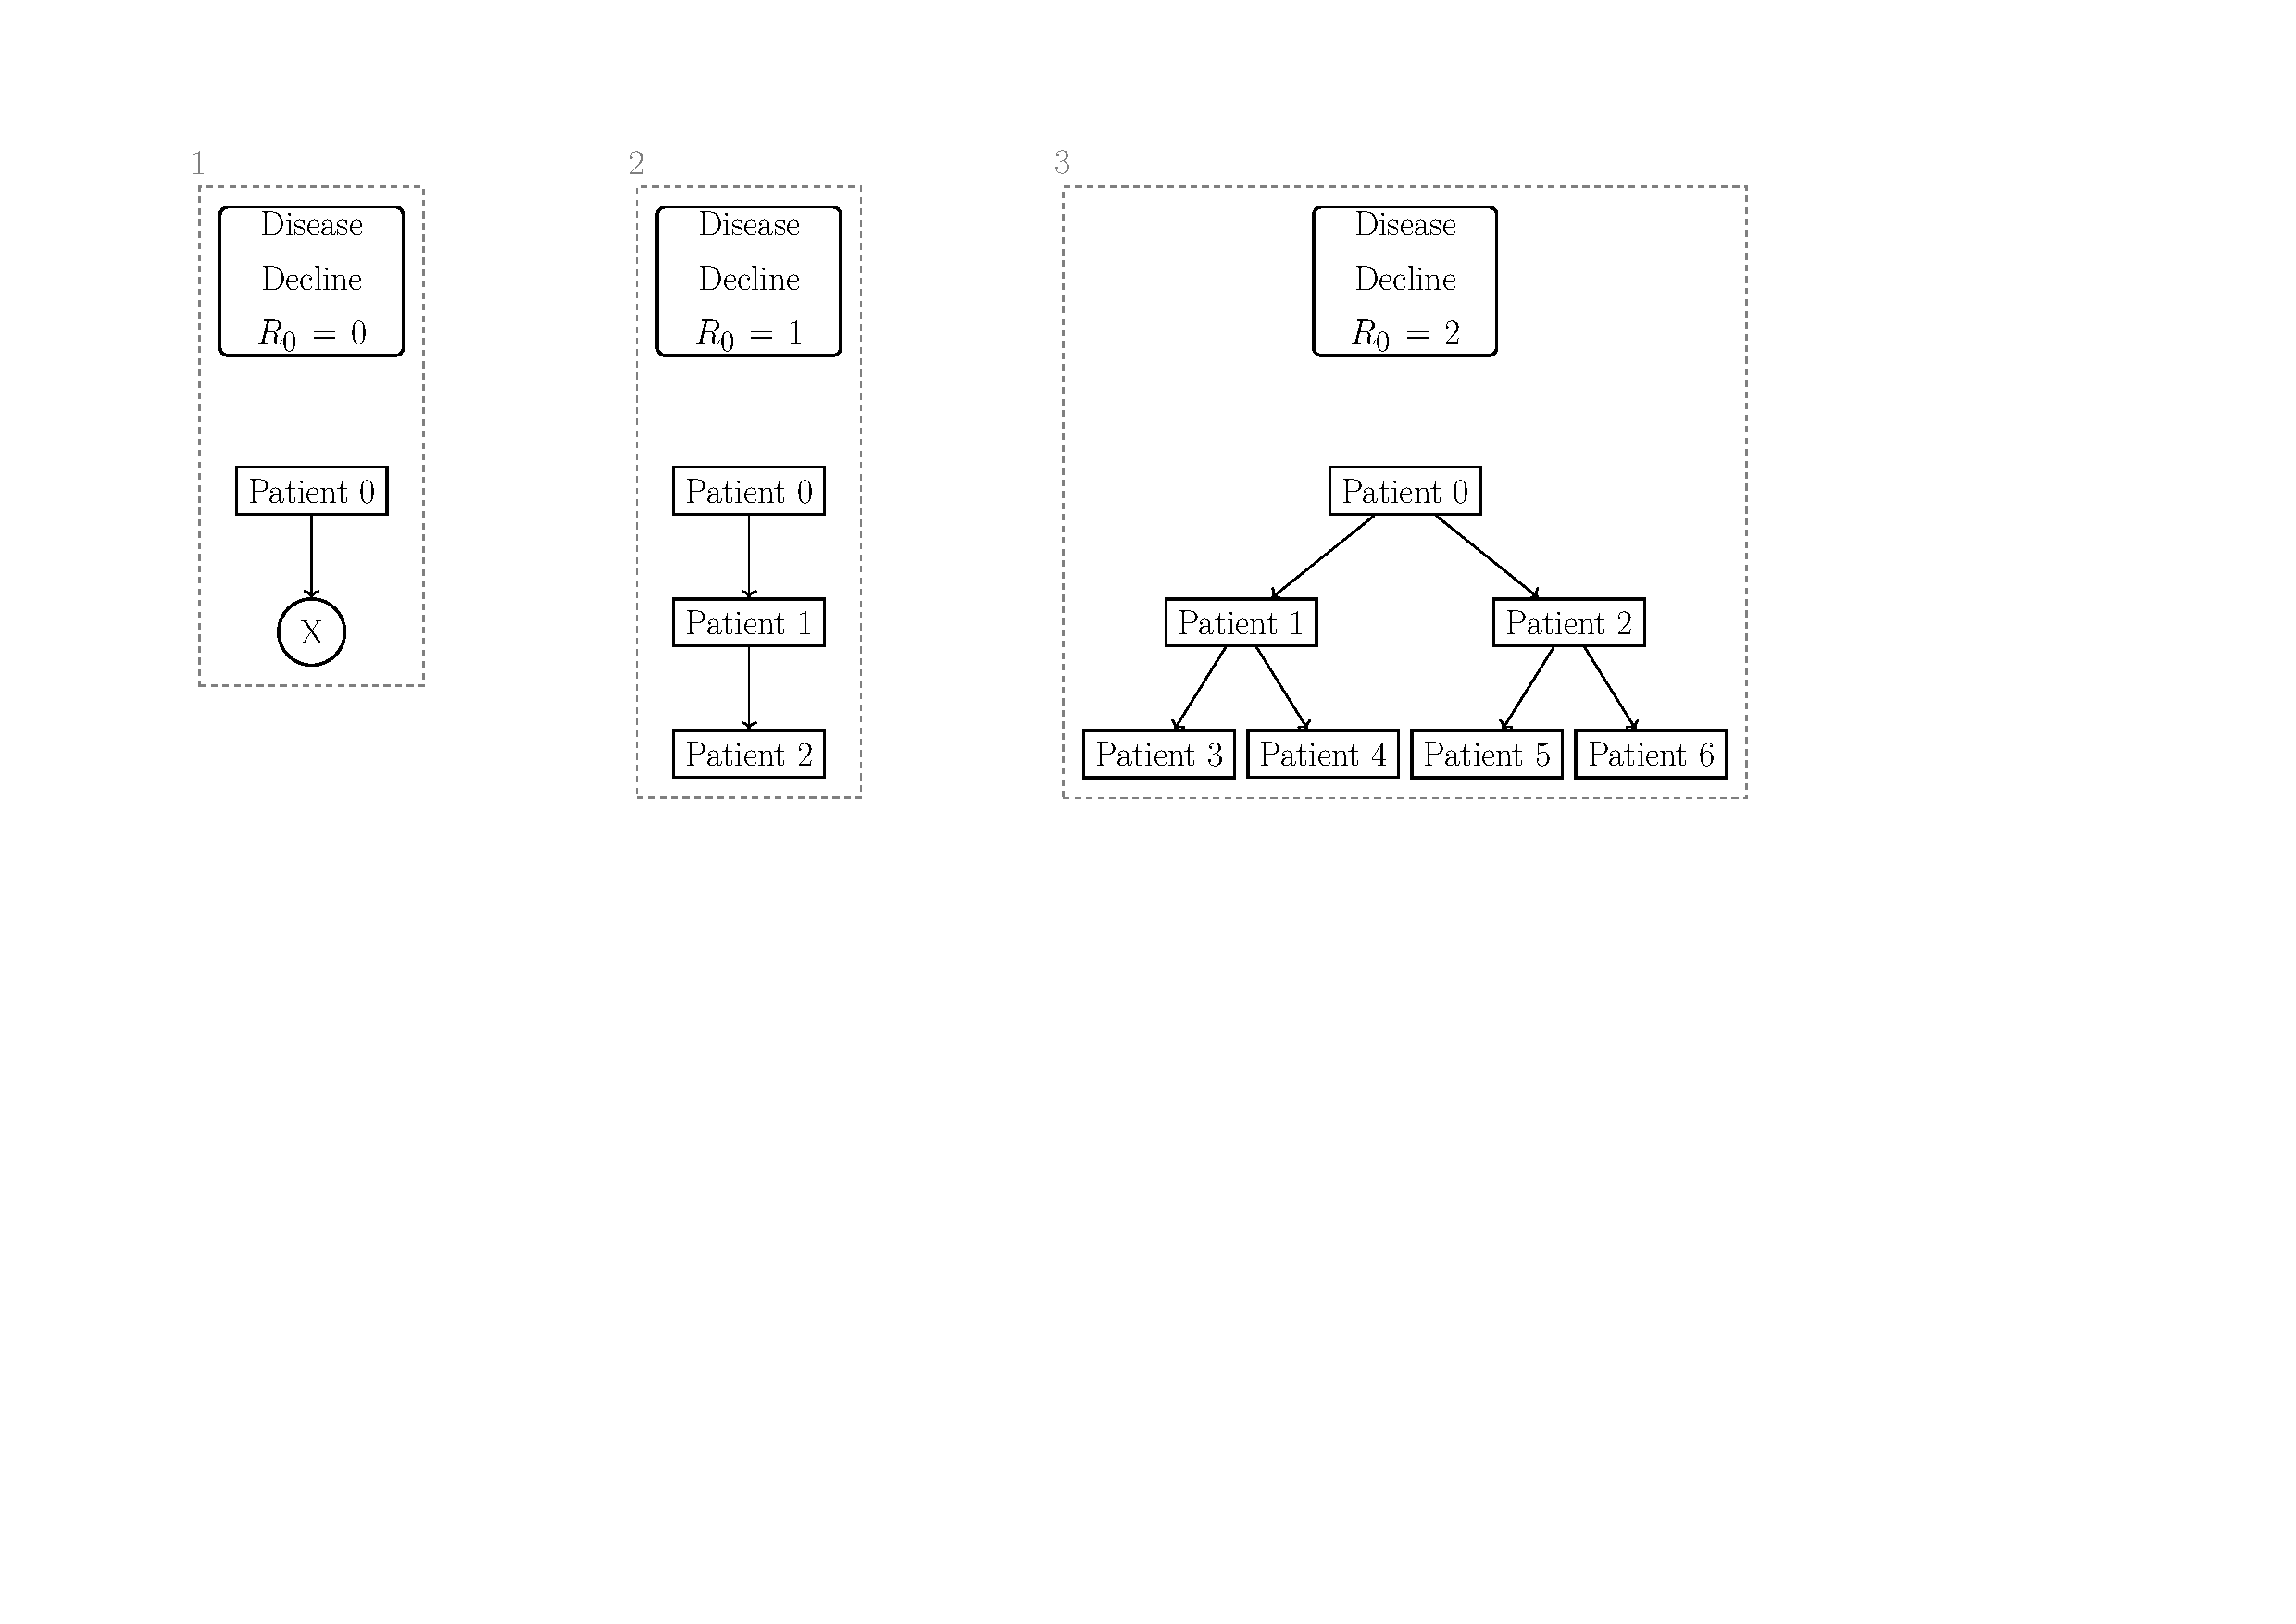
\includegraphics[width=14.25cm,height=6.5cm]{figures/modlingfig_2.pdf}}
    \caption{传染模型搭建}
\end{figure}

\vspace{-0.3cm}
其余参数sigma($\sigma$),mu($\mu$),gamma($\gamma$)均可以通过临床数据得出。

在各个国家和地区的参数都不相同,需要根据当地情况调整。如:
政府发布戴口罩、限制出行的政策可以降低易感者$S_0$,封锁城市减少人员流动会降低传染率b,疫苗的产生和治疗方法的成熟会显著提升治愈率g。

在特定的假设条件下,我们完成了SEIRD模型的构建:

\clearpage
\begin{figure}[!htp]
    \centerline{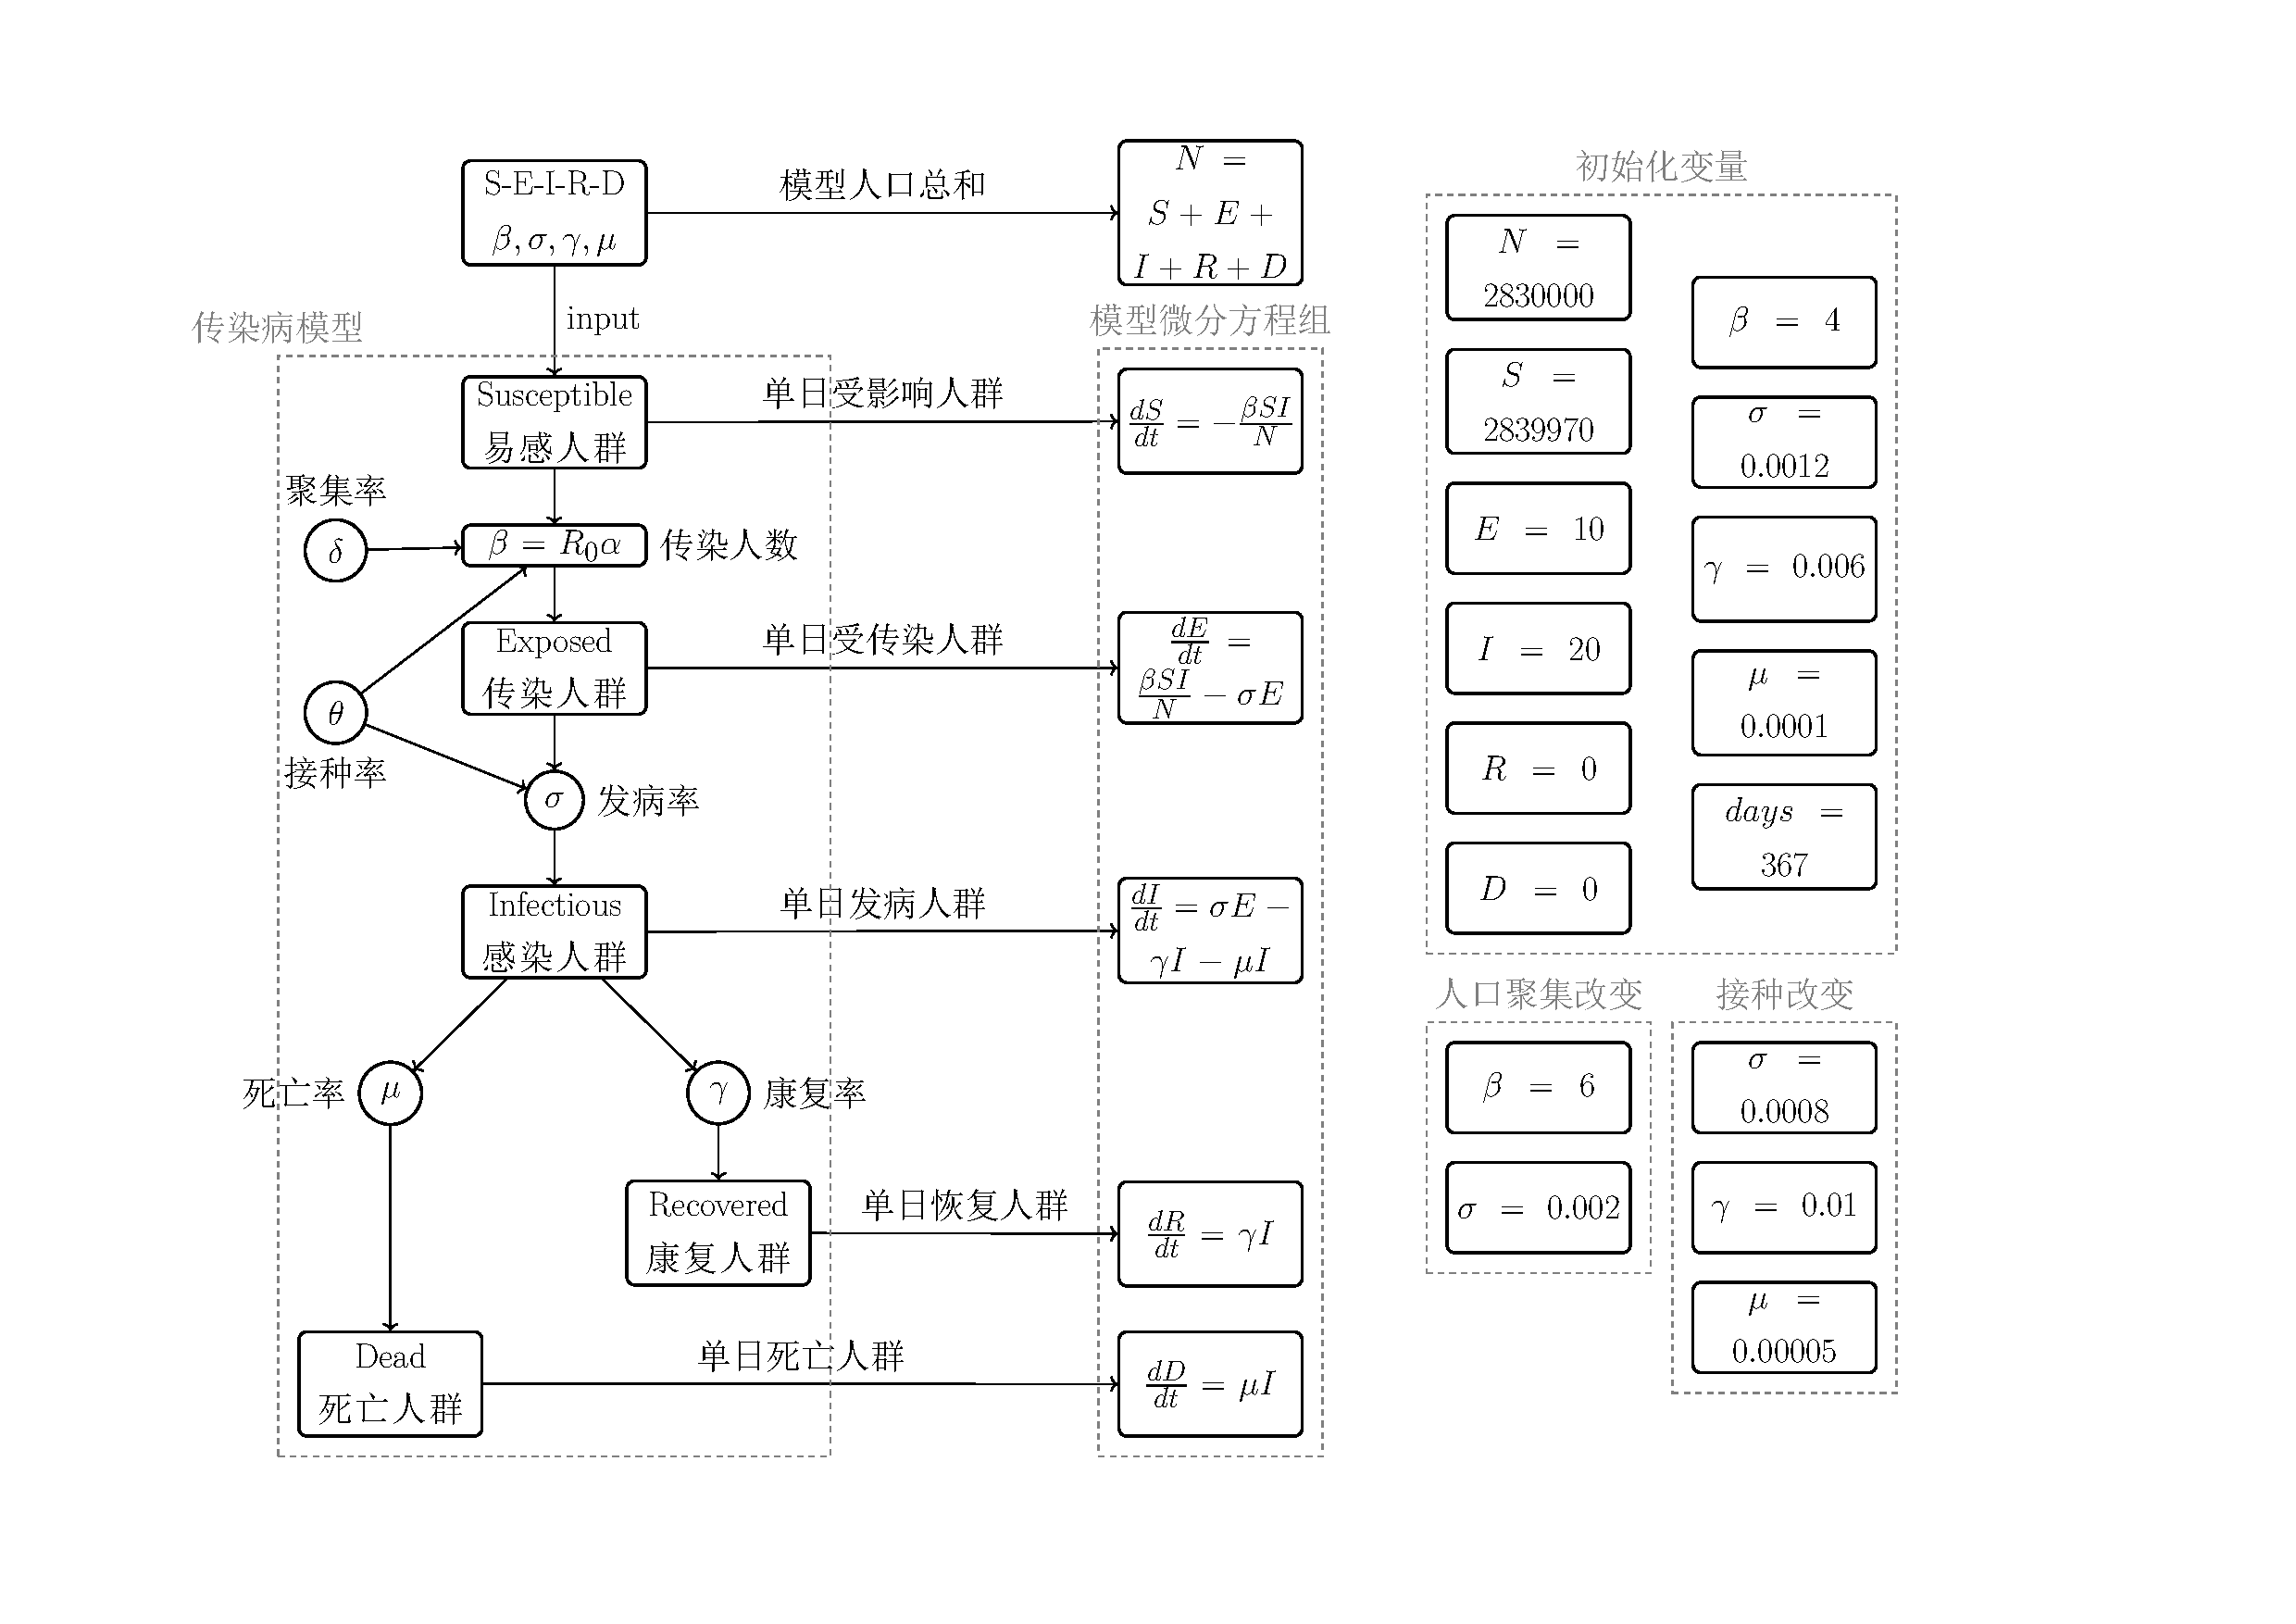
\includegraphics[width=13.596cm,height=10.2cm]{figures/modlingfig_1.pdf}}
    \caption{SEIRD模型流程图及超参参考值}
\end{figure}

\vspace*{-1.2cm}
\subsection{数据集的获取与筛选}

需要获取的目标数据集是阿肯色州的官方疫情统计数据,Microsoft Azure提供了COVID-19 Data Lake,包含了诸多地区的新冠肺炎相关数据集。我们在获取的数据集发现该数据集涵盖了一些对于本次建模工作不重要的信息,因此需要进行针对性筛选。对下载好的csv文件进行清洗,最终得到了2020年3月6日到2021年3月6日阿肯色州的疫情统计数据,并且获取了拟合模型所需要的参数。

\vspace*{-0.5cm}

\subsubsection{数据集的选取}
为建立SEIRD模型,在允许范围拥有数据类型较为符合要求的数据集。通过比对各官方网站上不同来源的数据。最终选定的数据集属性表如下

\begin{table}[!htp]
    \resizebox{\textwidth}{20mm}{
        \begin{tabular}{|c|c|c|c|c|c|}
            \hline
            属性                    & 名称             & 属性                           & 名称             & 属性                 & 名称             \\ \hline
            state                   & 州               & n\_icu\_currently              & ICU离开人数      & date\_checked        & 核对日期         \\ \hline
            positive                & 阳性             & on\_ventilator\_currently      & 使用呼吸机数     & death                & 死亡人数         \\ \hline
            negative                & 阴性             & on\_ventilator\_cumulative     & 总计使用呼吸机数 & hospitalized         & 住院人数         \\ \hline
            pending                 & 待检测           & recovered                      & 康复人数         & total\_test\_results & 总计检测人数     \\ \hline
            hospitalized\_currently & 当前住院人数     & data\_quality\_grade           & 数据可信度       & pos\_neg             & 检测阳阴性比例   \\ \hline
            hospitalized\_cumulated & 总计住院人数     & last\_update\_et               & 最近更细日期     & fips                 & 联邦信息管理     \\ \hline
            death\_increase         & 单日新增死亡人数 & hospitalized\_increase         & 单日新增住院人数 & negative\_increase   & 单日新增阴性人数 \\ \hline
            positive\_increase      & 检测阳性人数     & total\_test\_results\_increase & 单日新增检测数   & fips\_code           & 管理代号         \\ \hline
        \end{tabular}}
    \caption{数据集属性浏览表}
\end{table}

\clearpage
\subsubsection{数据集的清洗}
\begin{enumerate}
    \item[A] 相似值处理\\
          很多特征值之间具有相关性,这些特征并不需要全部关注。比如death, death\_increase,在该模型的处理过程中只需要关注death值。
    \item[B] 无关值处理\\
          有一些变量在该模型中并没有影响效用。比如positive、negative、negative\_increase、positive\_increase,这些本身并不需要被关注,因此可以排除在外。
    \item[C] 密切值处理\\
          我们是针对一个特定地区(例如本队选取阿肯色州进行分析),因此在state类别的数据我们只需要筛选标注AR的数据行。
\end{enumerate}
\vspace{-0.5cm}
\subsubsection{人工检查}
人工提取的过程较为繁琐,主观性较强,但是人工提取可以保证模型数据选取的准确性,在对庞大数据进行降维的过程,人工往往是比较有效的方法。
通过进行缺失值统计,利用零值进行填充,利用绘图函数进行历史数据的绘制
\vspace{-0.5cm}
\subsection{调整模型参数}
\noindent
经过上述步骤,获得的最终分析数据属性如下
\begin{enumerate}
    \item date:时间记录
    \item positive:单日病毒检测阳性人群数量
    \item recovered:单日康复人群数量
    \item death:单日死亡人群数量
\end{enumerate}
根据疫情的发展趋势,调整比对得出初始数据
\vspace{-0.5cm}
% \clearpage
\subsection{代码解释}
\begin{minted}
    [
    numbers = left,
    linenos,
    numbersep=2pt,
    baselinestretch=1.2,
    fontsize=\footnotesize,
    breaklines,
    frame=single
    ]
    {python}
# 微分方程模型求解
def ode_model(z, t, beta, sigma, gamma, mu):
    S, E, I, R, D = z           # z为数组装载了5个元素
    N = S + E + I + R + D       # 总人数
    dS/dt = -beta * S * I / N
    dE/dt = beta * S * I / N - sigma * E
    dI/dt = sigma * E - gamma * I - mu * I
    dR/dt = gamma * I
    dD/dt = mu * I
    return [dS/dt, dE/dt, dI/dt, dR/dt, dD/dt]
\end{minted}

\begin{minted}
    [
    numbers = left,
    linenos,
    numbersep=2pt,
    baselinestretch=1.2,
    fontsize=\footnotesize,
    breaklines,
    frame=single
    ]
    {python}
# scipy使用odeint函数求解微分方程
def ode_solver(t, initial_conditions, params):
    initE, initI, initR, initN, initD = initial_conditions
    beta, sigma = params['beta'].value, params['sigma'].value
    gamma, mu = params['gamma'].value, params['mu'].value
    initS = initN - (initE + initI + initR + initD)
    res = odeint(ode_model, [initS, initE, initI, initR,initD], t, args=(beta, sigma, gamma, mu))
    return res
\end{minted}


\begin{minted}
    [
    numbers = left,
    linenos,
    numbersep=2pt,
    baselinestretch=1.2,
    fontsize=\footnotesize,
    breaklines,
    frame=single
    ]
    {python}
# 演示效果动态调参
def main(initE, initI, initR, initD, initN, beta, sigma, gamma, mu, days, param_fitting):
    initial_conditions = [initE, initI, initR, initN, initD]
    params['beta'].value,params['sigma'].value,params['gamma'].value,params['mu'].value = [beta,sigma,gamma,mu]
    tspan = np.arange(0, days, 1)   # 横坐标
    sol = ode_solver(tspan, initial_conditions, params) # 返回二维数组,6列
    S, E, I, R, D = sol[:, 0], sol[:, 1], sol[:, 2], sol[:, 3], sol[:, 4]   # 前面所有行,逗号后面是所有列

    fig = go.Figure()   # 动态图,绘图
    fig1 = go.Figure()
    if not param_fitting:   # 对应按钮,改变或不改变
        fig.add_trace(go.Scatter(x=tspan, y=S, mode='lines+markers', name='Susceptible'))
        fig.add_trace(go.Scatter(x=tspan, y=E, mode='lines+markers', name='Exposed'))
        fig.add_trace(go.Scatter(x=tspan, y=I, mode='lines+markers', name='Infected'))
        fig.add_trace(go.Scatter(x=tspan, y=R, mode='lines+markers',name='Recovered'))
        fig.add_trace(go.Scatter(x=tspan, y=D, mode='lines+markers',name='Death'))
        fig1.add_trace(go.Scatter(x=tspan, y=I, mode='lines+markers', name='Infected'))
        fig1.add_trace(go.Scatter(x=tspan, y=R, mode='lines+markers',name='Recovered'))
        fig1.add_trace(go.Scatter(x=tspan, y=D, mode='lines+markers',name='Death'))
    if param_fitting:
        fig.add_trace(go.Scatter(x=tspan, y=df_temp2.positive, mode='lines+markers', name='Infections Observed', line=dict(dash='dash')))
        fig.add_trace(go.Scatter(x=tspan, y=df_temp2.recovered, mode='lines+markers', name='Recovered Observed', line=dict(dash='dash')))
        fig.add_trace(go.Scatter(x=tspan, y=df_temp2.death, mode='lines+markers', name='Deaths Observed', line=dict(dash='dash')))

    if days <= 30:  # 对时长进行步长设置
        step = 1
    elif days <= 90:
        step = 7
    else:
        step = 30

    # 横坐标和纵坐标名称图片宽度高度
    fig.update_layout(title='Simulation of SEIRD Model', xaxis_title='Day', yaxis_title='Counts', title_x=0.5, width=900, height=600)
    fig.update_xaxes(tickangle=-90, tickformat = None, tickmode='array', tickvals=np.arange(0, days + 1, step))
    fig1.update_layout(title='SEIRD test',xaxis_title='Day', yaxis_title='Counts', title_x=0.5, width=1000, height=600)
    if not os.path.exists("images"):
        os.mkdir("images")  # 创建图片所在文件夹
        fig.write_image("images/seird_simulation.png")  # 生成图像
        fig.show()   # 展示图像
\end{minted}
% \vspace*{-0.7cm}
\subsection{分析阿肯色州COVID\_19病毒的传播情况}
% \vspace*{-0.3cm}
\subsubsection{初步分析拟合}
% \vspace*{-0.7cm}

\clearpage
\begin{figure}[!htp]
    \centerline{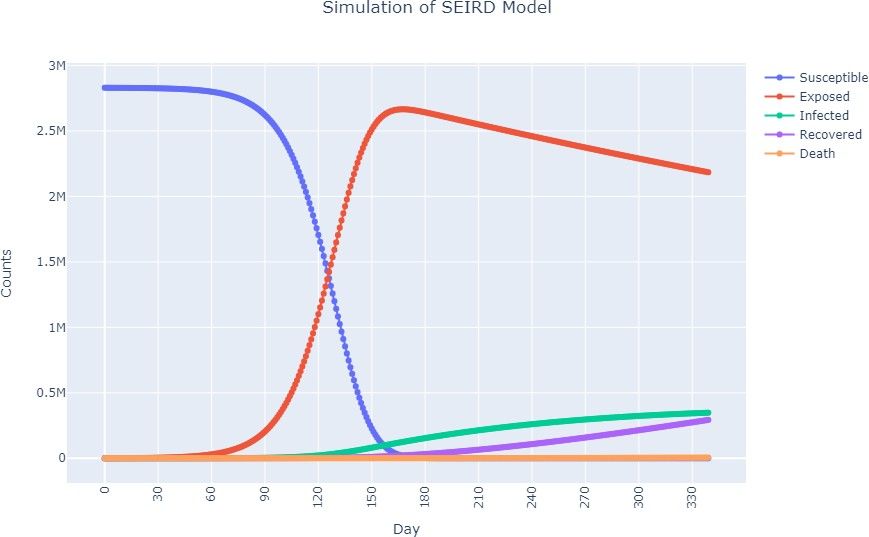
\includegraphics[width=15.65cm,height=9.67cm]{figures/参数拟合.png}}
    \caption{参数调整可视化图像}
    % 13.04 8.06
\end{figure}

% \clearpage
\vspace*{-1.2cm}
\subsubsection{使用L-M算法进行优化}
连续历元权重变化公式:$\Delta W_{m}=-\dfrac{d_{m}}{(H_{m}+e^{\lambda}I)}$
在python中使用lmfit库中的最小化模块,并运用Levenberg-Marquardt算法来最小化
非线性最小二乘。对残差编码进行并将其限制在最小值。优化完成后,生成对应模型对比图和优化后的模型参数:

\vspace*{-0.25cm}

\begin{figure}[!htp]
    \centerline{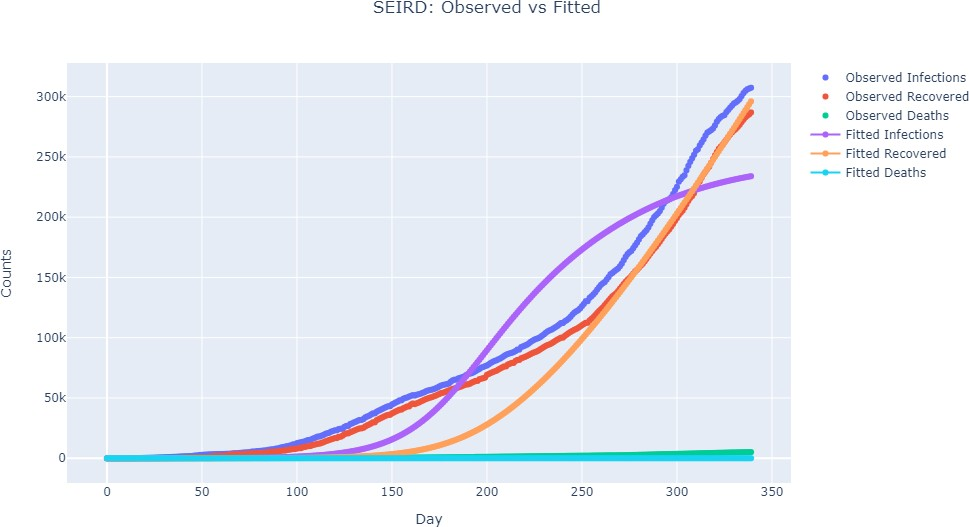
\includegraphics[width=13.26cm,height=7.49cm]{figures/finalnihe.png}}
    \caption{优化参数可视化对比图}
\end{figure}

\vspace{-0.3cm}
% 12.06 6.81
\begin{minted}
    [
    numbers = left,
    linenos,
    numbersep=2pt,
    baselinestretch=1.2,
    fontsize=\footnotesize,
    breaklines,
    frame=single
    ]
    {python}
[[Variables]]
beta:   2.62206596  +/- 0.07065303  (2.69%) (init = 4)
sigma:  0.00119439  +/- 2.0997e-05  (1.76%) (init = 0.0012)
gamma:  0.01052104  +/- 1.6378e-04  (1.56%) (init = 0.006)
mu: 5.4349e-11  +/- 1.8250e-05  (33578621.44%) (init = 0.0001)
[[Correlations]] (unreported correlations are < 0.100)
C(beta, sigma) = -0.953     C(beta, gamma) = -0.550     C(sigma, gamma) = 0.530
C(sigma, mu) = -0.389       C(beta, mu) = 0.213
\end{minted}
\clearpage
\subsubsection{指标计算补充}
使用优化参数调用定义后的ode\_solver计算MAE(平均绝对误差)和RMSE
(均方根误差)
\begin{minted}
    [
    numbers = left,
    linenos,
    numbersep=2pt,
    baselinestretch=1.2,
    fontsize=\footnotesize,
    breaklines,
    frame=single
    ]
    {python}
Fitted MAE                                          Fitted RMSE
Infected: 20794.332654685975                        Infected: 27499.729191344883
Recovered: 14536.028287085463                       Recovered: 21159.039391924664
Dead: 1348.6585045293205                            Dead: 2000.0961938063565
\end{minted}
\subsubsection{结论总结}
\begin{enumerate}
    \item 阿肯色州的预测曲线的拐点远早于实际数据,这说明防疫措施并不到位,图像很晚达到拐点说明该地区的确诊人数仍然将快速增长,需要政府发布更有效的政令,民众更遵守疫情防控规则,才能使疫情拐点更早到来。
    \item 阿肯色州的治愈人数曲线从100天到150天明显高于预测曲线,说明医疗物资的供给提高和疫情防治的方法成熟使得治愈人数上升;但150天后曲线又相互吻合,推测是病毒变异的出现使得患者更难被治愈。
    \item 阿肯色州的死亡人数始终高于预测曲线,说明医疗防治手段还需要进一步整体提升。
\end{enumerate}

\clearpage
\section{人类移动和聚集行为对新冠病毒传播的影响}
\subsection{阿肯色州人群移动与聚集行为调查分析}
新冠病毒流行改变着人们的流动方式,需要流行病学模型来捕捉这些流动性变化对严重急性呼吸系统综合症冠状病毒传播的影响。为了应对新冠肺炎危机,各国都颁布了国内禁流命令,以减少个人之间的联系,并减缓SARS-新冠肺炎-29的传播。

将流行病学模型与移动模型相结合,不仅能够准确地适应观察到的病例计数,而且能够进行详细的分析,从而对covid-19提供更有效和更公平的政策反应信息。

美国阿肯色州人群移动性在 2020 年 3 月急剧下降。例如,在 3 月的第一周和
2020 年 4 月的第一周之间,阿肯色州的整体 POI 访问量下54.7\%。

查阅资料得知,低收入人群具有更高的传播率,但是人均访问量的差异并不能完全解释感染差异。以下分析提供用于分析流动性减少或增多、重新开放移动计划和聚集
人口差异的实验程序的详细信息。

\subsection{分析现有图像推断病毒传播}
结论:发病率随聚集人数增多/移动人群计数增加而增大;传染人数随之上升。采用控制变量进行验证。

初始图像在原有的图像上进行调整,考虑到新冠病毒变异快、爆发猛,即使在封闭区域也会自发增强感染性,因此在原有预测数据的基础上进一步感染人数,以贴合疫情本身特性。
\begin{figure}[!htp]
    \centering
    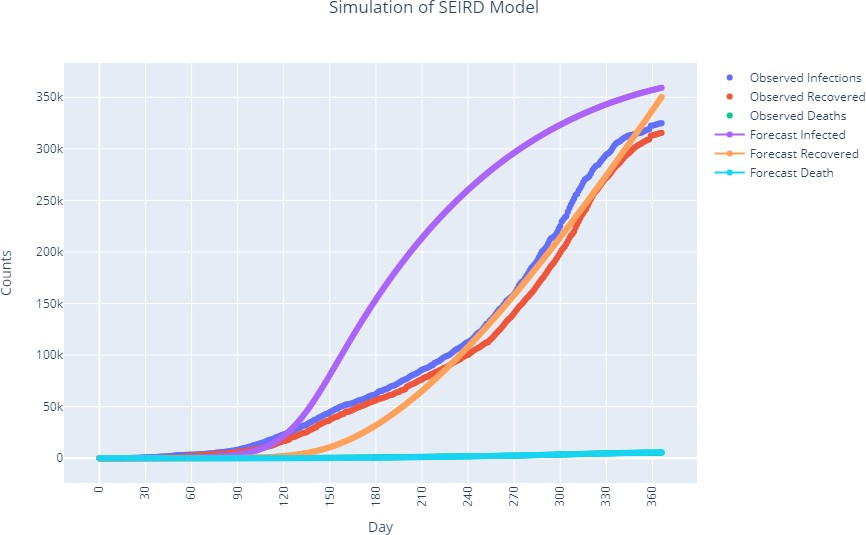
\includegraphics[width=15.6cm,height=9.64cm]{figures/original.png}
    \caption{原始参考图}
\end{figure}

\clearpage
\begin{figure}[!htb]
    \centering
    \subfloat[sigma($\sigma$)=0.0016]{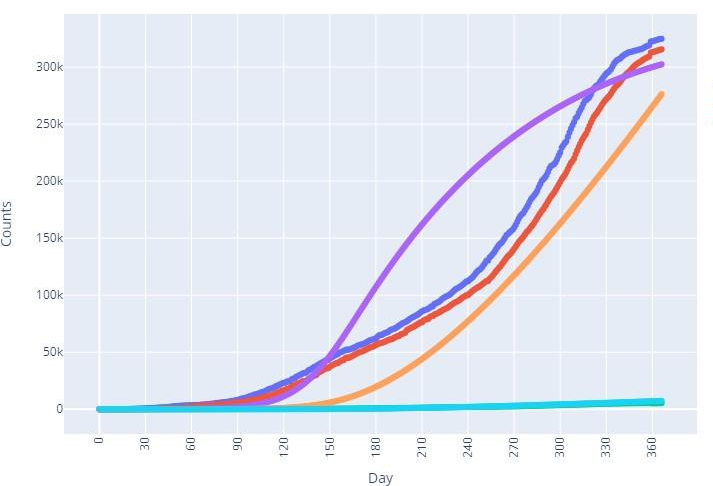
\includegraphics[width=0.49\linewidth]{figures/sigmma0.0016.png}}
    \hfill
    \subfloat[sigma($\sigma$)=0.0014]{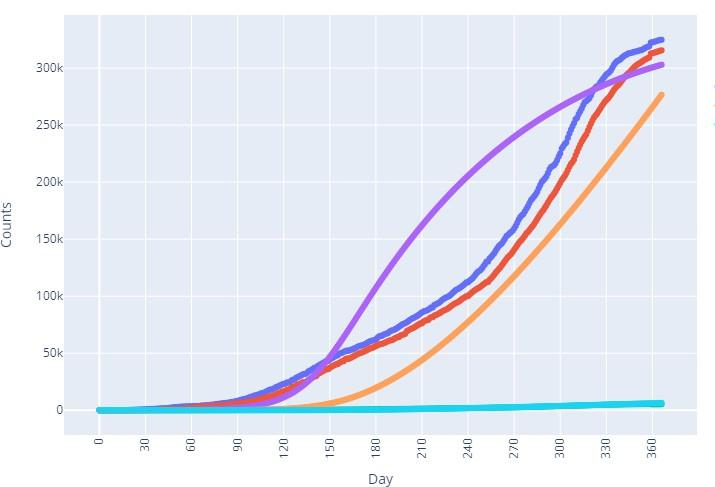
\includegraphics[width=0.49\linewidth]{figures/sigmma0.0014.png}} \\
    \subfloat[sigma($\sigma$)=0.0010]{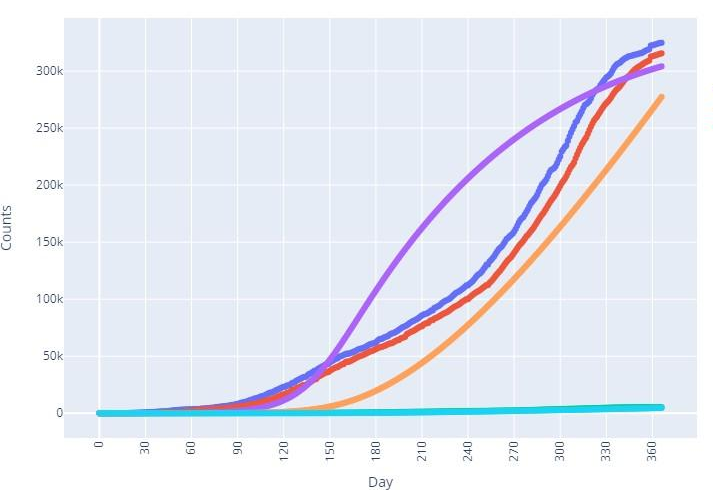
\includegraphics[width=0.49\linewidth]{figures/sigmma0.0010.png}}
    \hfill
    \subfloat[sigma($\sigma$)=0.0008]{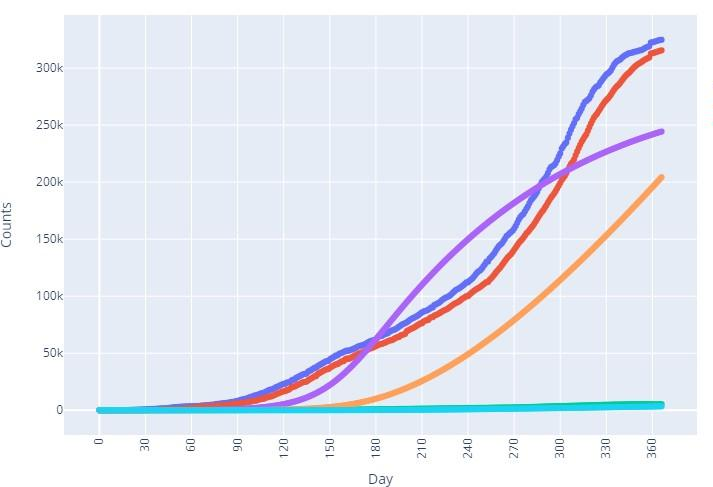
\includegraphics[width=0.49\linewidth]{figures/sigmma0.0008.png}}
    \caption{参数对比图}
\end{figure}
调整数据,进行控制变量分析。保持beta = 4不变,首先改变sigma,上调或下调。

已知原数据中我们控制sigma初值为0.0012,那么在增加到0.0014时代表发病率增高,而这是聚集人数增多/移动基数变大导致的。分析图像趋势可知,此时观测到的感染人数开始多于预测的感染人数。随着sigma值继续提高到0.0016,图像继续发⽣微小改变,感染人数观测值比预测值多了更多。

当sigma值减小到0.0010时,预测感染与观测感染都变少了。说明随着聚集人数和移动人群减少,感染数变小。随着sigma值降到更低的水平,预测感染与观测感染变得更少,并且产生图形上更⼤的变化。

综上,当仅仅考虑到发病率的时候,我们可以认为聚集程度和移动范围与发病率呈正相关。与此相对应的是,随着聚集和移动的人数提高,发病率变大。

\clearpage
\begin{figure}[!htb]
    \centering
    \subfloat[beta($\beta$)=10]{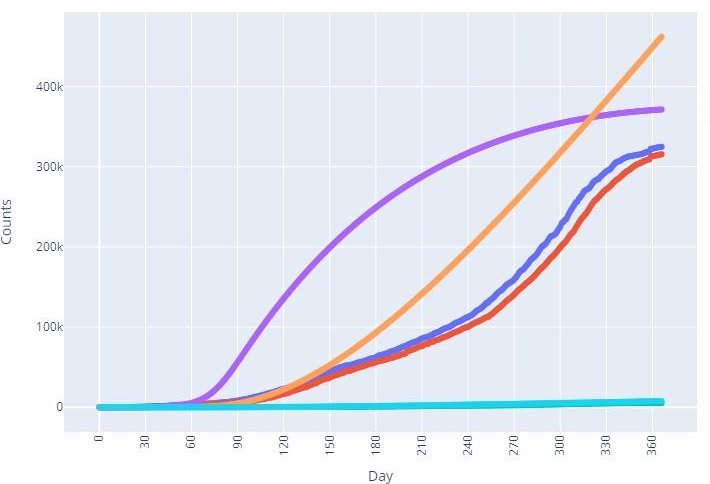
\includegraphics[width=0.49\linewidth]{figures/beta10.png}}
    \hfill
    \subfloat[beta($\beta$)=8]{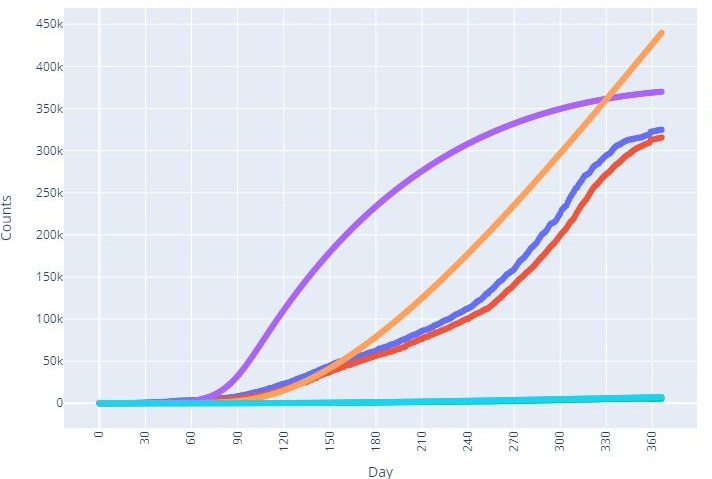
\includegraphics[width=0.49\linewidth]{figures/beta8.png}} \\
    \subfloat[beta($\beta$)=6]{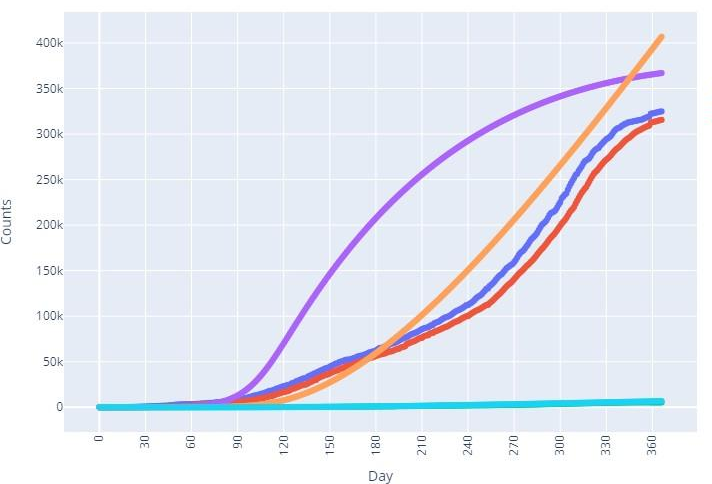
\includegraphics[width=0.49\linewidth]{figures/beta6.png}}
    \hfill
    \subfloat[beta($\beta$)=2]{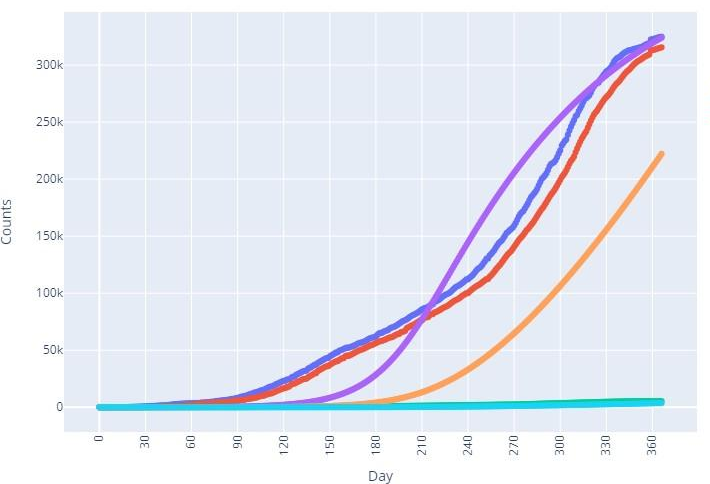
\includegraphics[width=0.49\linewidth]{figures/beta2.png}}
    \caption{参数对比图}
\end{figure}
调整数据,进行控制变量分析。保持sigma = 0.0012不变,改变beta,上调或下调。

已知原数据中我们控制beta初值为4,那么在增加到6/8/10时代表感染人数增加,这是聚集人数增多/移动基数变大导致的。

分析图像趋势可知,beta为6时观测到的感染人数略少于预测的感染人数;而随着beta值继续提高到8,图像继续发生改变,感染人数观测值持续变多,预测值持续变
多。beta提高到10时,毫无悬念地,感染人数的观测值和预测值都多于原值情况下观察值和预测值。
当beta值减小到2时,预测感染与观测感染都变少了。说明随着聚集人数和移动人群减少,感染数变小。

综上,当仅仅考虑到感染人数的时候,我们可以认为感染人数受到聚集程度和移动范围影响;也可以认为聚集程度和移动范围与感染人数呈正相关。与此相对应的是,随着聚集和移动的人数提⾼,感染人数增加。


\subsection{结论}
我们认为严格的疫情防控和控制移动范围、控制聚集等活动对COVID-19的传染起到了良性作用,为了减小感染病毒可能性,减少大型集会、减少跨区域移动对防控病毒的传播起到有效作用。

\clearpage
\section{疫苗存在的情况下对地区疫情进行分析}
\subsection{分析相关参数改变}
以色列是人均接种率最高的国家之一。根据以色列卫生部自然研究报告显示,间隔
21天的两剂给药方案可以提供95\%的保护率;在第一剂后14-20天和第二剂后7天的疗效分别为46\%和92\%。
在接种人群方面,青少年、服役年轻人和重症患者拥有疫苗优先权。数据显示,与晚期接种疫苗的城市相比,
早期接种疫苗的城市的COVID-19病例数和60岁及以上人群的住院人数下降幅度更大、更早;与峰值相比,
早期接种疫苗的城市病例减少了88\%,重症住院减少了79\%,而在接种疫苗较晚的城市,病例减少了78\%,
重症住院减少了66\%。因此疫苗可以显著降低发病率、死亡率,大幅提升治愈率;另一方面,封锁城市、
禁止群众集会可以显著抑制人口流动,有利于组织疫苗接种,可以降低病毒的传染率和人群的发病率。

但是疫苗的接种需要群众的意愿支持,这也导致民众对于疫苗的态度会影响疫苗在整个地区发挥的作用,
而科学研究显示一种新型疫苗至少需要55\%的人口接受才能提供对社会群体较全面的保护。
如今社交媒体上流传着关于新冠肺炎病情的虚假信息,例如5G移动网络会随着疫苗进入人体、疫苗会导致人死亡等,
会在一定程度上影响地区的接种⼯作。在英美地区,分别有54.1\%和42.5\%的受访者表示他们“绝对”接受疫苗以保护
自己,有6\%和15\%表示他们“绝对不会”接受疫苗。另一方面,地区的经济水平和教育
水平也会对疫苗接种率造成影响,影响的因素包括疫苗供给和群众对疫苗的认知水平等。

\begin{table}[!htp]
    \resizebox{\textwidth}{24mm}{
        \begin{tabular}{|c|c|c|c|}
            \hline
            疫苗名称                   & 辉瑞新冠肺炎疫苗      & Moderna新冠肺炎疫苗 & 强生新冠肺炎疫苗  \\ \hline
            疫苗类型                   & mRNA疫苗              & mRNA疫苗            & 腺病毒载体疫苗    \\ \hline
            三期疫苗实验率             &
            \begin{tabular}[c]{@{}c@{}}95\%\\ (16-55岁为95.6\%)\\ (56岁以上为93.7\%)\end{tabular} &
            \begin{tabular}[c]{@{}c@{}}94.1\%\\ (18-64岁为95.6\%)\\ (65岁以上为86.4\%)\end{tabular} &
            \begin{tabular}[c]{@{}c@{}}86\%\\ (预防中重度有效率平均为66.1\%)\end{tabular}                                                                   \\ \hline
            存放温度                   &
            \begin{tabular}[c]{@{}c@{}}$-80^{\circ}$C至$-60^{\circ}$C\\ ($2^{\circ}$C至$8^{\circ}$C可存放5日)\end{tabular} &
            \begin{tabular}[c]{@{}c@{}}$-25^{\circ}$C至$-15^{\circ}$C\\ ($-80^{\circ}$C至$-60^{\circ}$C可存放30日)\\ ($8^{\circ}$C至$25^{\circ}$C可存放12小时)\end{tabular} &
            \begin{tabular}[c]{@{}c@{}}$-20^{\circ}$C以下可存放两年\\ ($2^{\circ}$C至$8^{\circ}$C可存放3个月)\end{tabular}                                                                   \\ \hline
            使用时间                   & 稀释后常温6小时内用完 & 开封后6小时内用完   & 开封后6小时内用完 \\ \hline
            有效期                     & 6个月以上             & 6个月以上           & 6个月以上         \\ \hline
            说明                       & 无                    & 无                  & 无                \\ \hline
        \end{tabular}}
    \caption{国外主流接种疫苗数据}
\end{table}

各州从有效率角度考虑,会尽可能多选择辉瑞和Moderna疫苗,而这两种疫苗的有效率非常接近,因此在调整参数上忽略细微区别。

\clearpage
\subsection{分析疫情发展情况}
根据Our World In Data可查到的阿肯色州疫苗接种率,在2020年1月份该州正式启动了疫苗接种工作,
在2月初疫苗接种率达到10\%,在3月初达到20\%,4月初达到30\%。而我们的疫情数据起始日期是
2020年3月6日至2021年3月6日,在该范围内对接种和聚集情况进行分析,适当调整参数,观察原数据和预测数据。

在原始数据中,政府在一定程度上限制人员聚集和移动,且可以实现疫苗在人群中的一定程度接种。对比图象如下:
\begin{figure}[!htb]
    \centering
    \subfloat[SEIRD模型模拟]{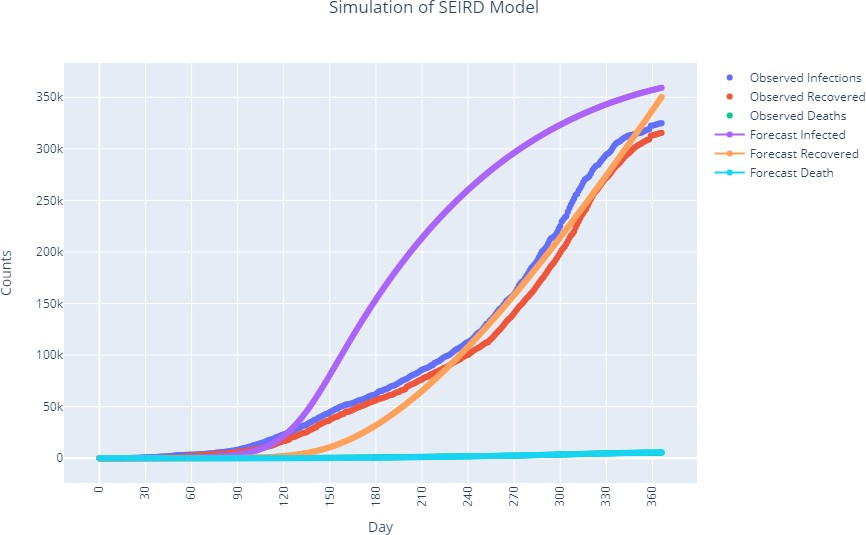
\includegraphics[width=0.5\linewidth]{figures/original.png}}
    \hfill
    \subfloat[模拟仿真感染数据对比]{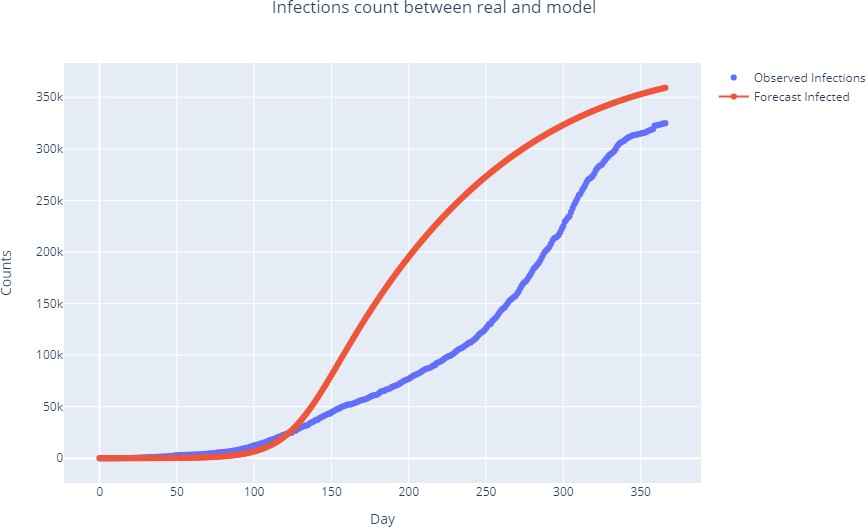
\includegraphics[width=0.5\linewidth]{figures/infections1.png}} \\
    \subfloat[模拟仿真康复数据对比]{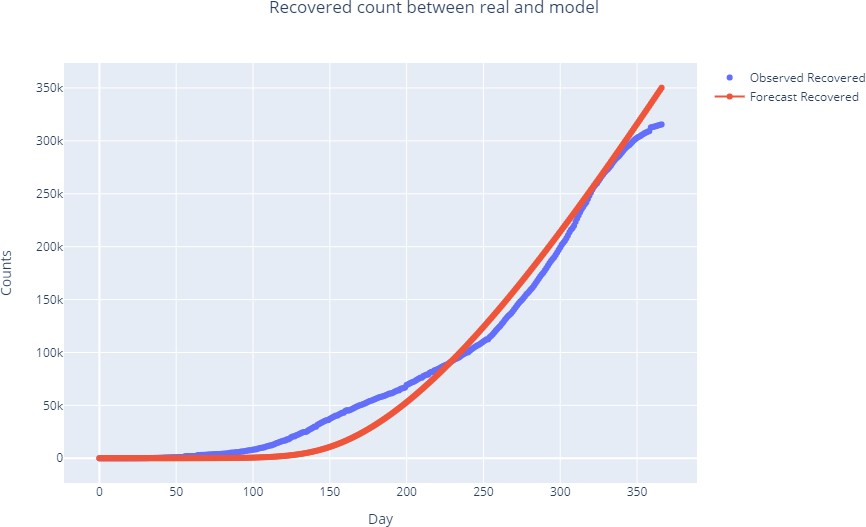
\includegraphics[width=0.5\linewidth]{figures/recovered1.png}}
    \hfill
    \subfloat[模拟仿真死亡数据对比]{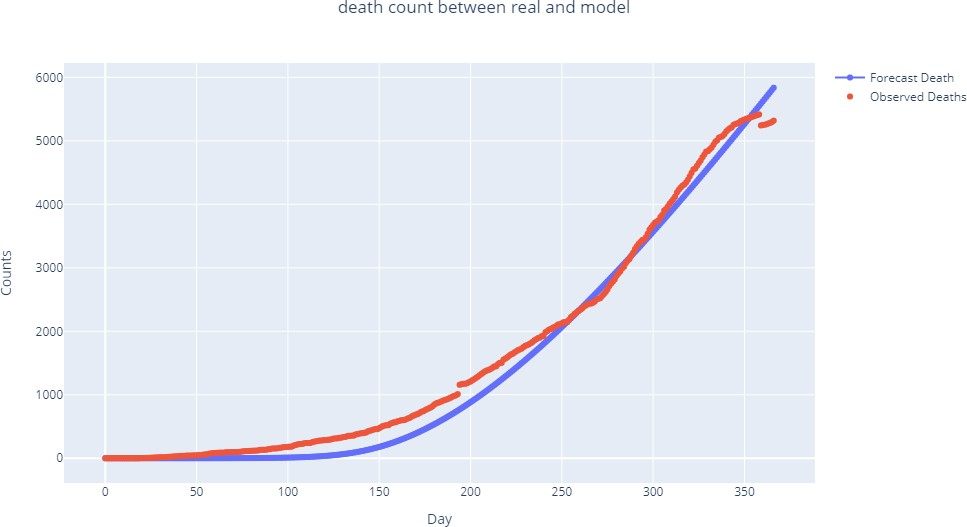
\includegraphics[width=0.5\linewidth]{figures/death1.png}}
    \caption{模型实际数据对比图}
\end{figure}

\begin{table}[!htp]
    \resizebox{\textwidth}{26mm}{
        \begin{tabular}{|c|c|c|c|}
            \hline
            疫情发展趋势               & 疫情得到有效控制                                              & 疫情未得到控制 & 疫情的实际发展情况 \\ \hline
            传染人数(beta)             & 1                                                             & 6              & 4                  \\ \hline
            发病率(sigma)              & 0.0008                                                        & 0.002          & 0.0012             \\ \hline
            康复率(gamma)              & 0.001                                                         & 0.004          & 0.0034             \\ \hline
            死亡率(mu)                 & 0.0005                                                        & 0.0008         & 0.0006             \\ \hline
            群众活动                   &
            \begin{tabular}[c]{@{}c@{}}民众不聚集\\ 自发接种疫苗\end{tabular} &
            \begin{tabular}[c]{@{}c@{}}民众大范围聚集\\ 极少数人接种疫苗\end{tabular} &
            \begin{tabular}[c]{@{}c@{}}民众保持日常活动\\ 进一半人接种疫苗\end{tabular}                                                                                                       \\ \hline
            政府管控                   &
            \begin{tabular}[c]{@{}c@{}}严格控制人员聚集活动\\ 疫苗储备充足\end{tabular} &
            \begin{tabular}[c]{@{}c@{}}几乎不限制人员聚集活动\\ 无疫苗储备\end{tabular} &
            \begin{tabular}[c]{@{}c@{}}发布公告鼓励居家\\ 少量疫苗储备\end{tabular}                                                                                                       \\\hline
            说明                       & \multicolumn{3}{c|}{除上述参数具有差异,其余模型参数保持不变}                                       \\ \hline
        \end{tabular}}
    \caption{疫情模拟情况参数对比表}
\end{table}
\clearpage
假设在聚集且不接种疫苗的情况下,政府几乎不限制人员聚集和移动,且只有极小
一部分人接种疫苗。对比图像如下:

\vspace{-0.4cm}
\begin{figure}[!htb]
    \centering
    \subfloat[SEIRD模型模拟]{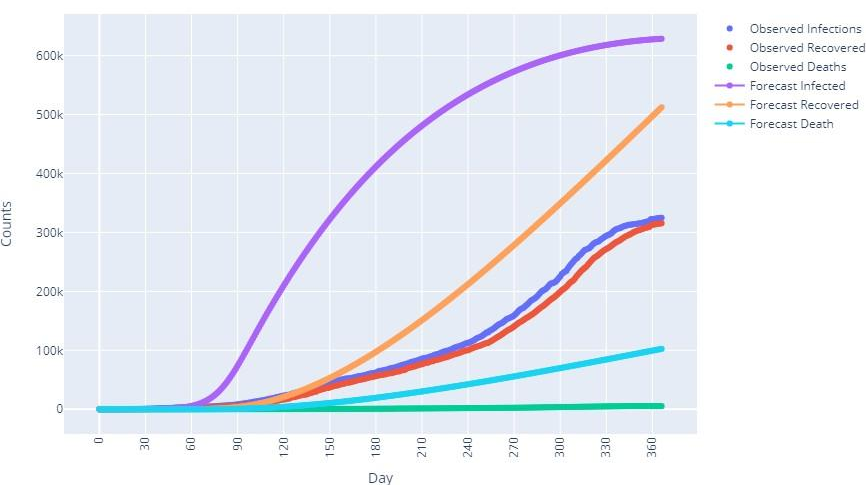
\includegraphics[width=0.5\linewidth]{figures/simulate_worse.png}}
    \hfill
    \subfloat[模拟仿真感染数据对比]{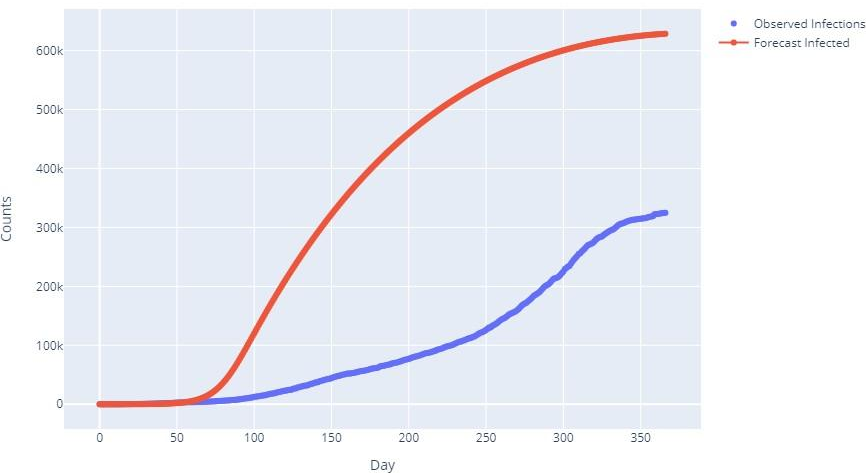
\includegraphics[width=0.5\linewidth]{figures/worse_infections.png}} \\
    \subfloat[模拟仿真康复数据对比]{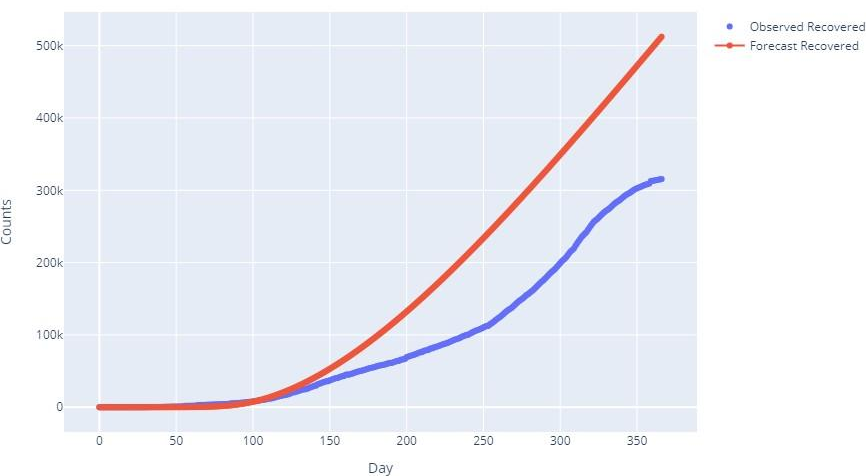
\includegraphics[width=0.5\linewidth]{figures/worse_recovered.png}}
    \hfill
    \subfloat[模拟仿真死亡数据对比]{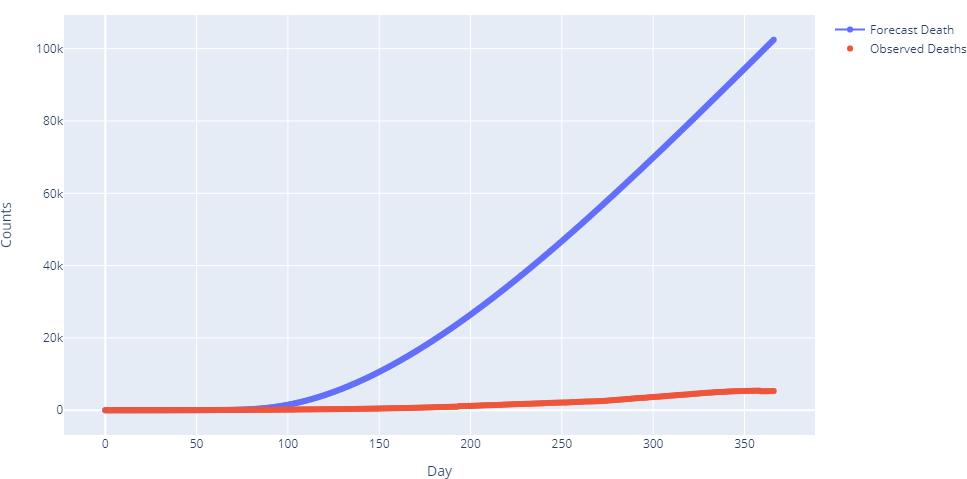
\includegraphics[width=0.5\linewidth]{figures/worse_death.png}}
    \caption{疫情恶化模型实际数据对比图}
\end{figure}

\vspace{-0.5cm}
假设在不聚集且接种疫苗的情况下,政府严格控制人员聚集和移动,群众自发接种疫苗,
疫苗储备充足。对比图像如下:
\vspace{-0.4cm}
\begin{figure}[!htb]
    \centering
    \subfloat[SEIRD模型模拟]{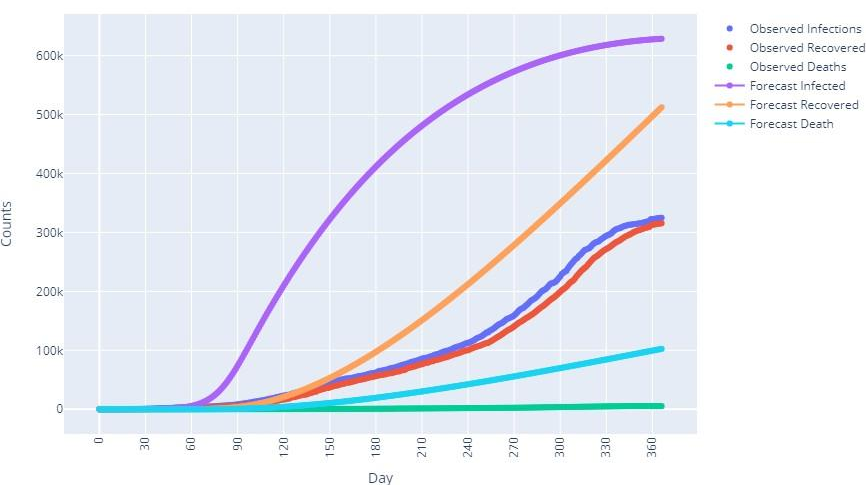
\includegraphics[width=0.5\linewidth]{figures/simulate_worse.png}}
    \hfill
    \subfloat[模拟仿真感染数据对比]{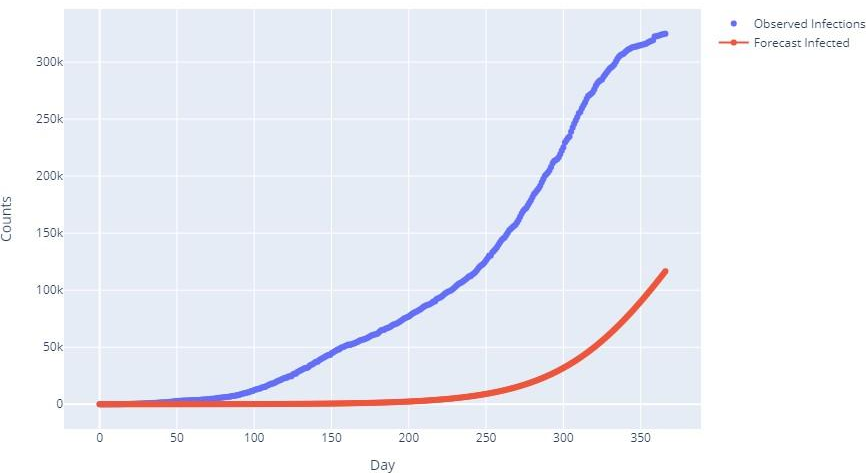
\includegraphics[width=0.5\linewidth]{figures/better_infections.png}} \\
    \subfloat[模拟仿真康复数据对比]{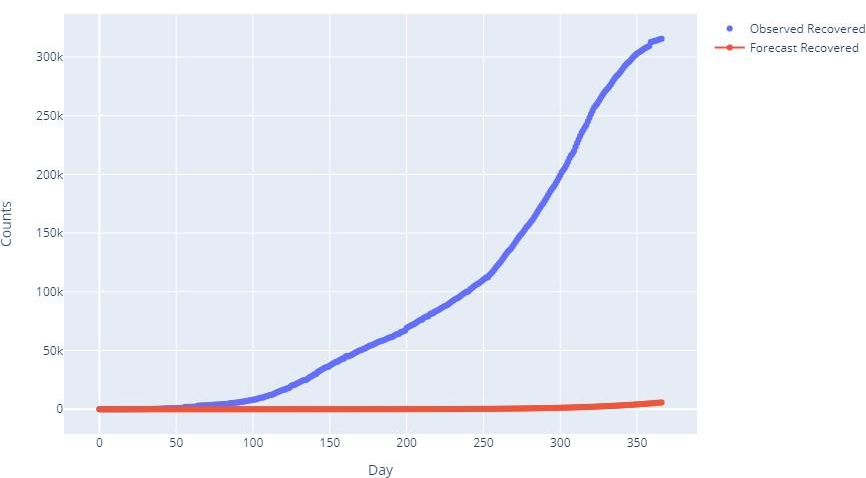
\includegraphics[width=0.5\linewidth]{figures/better_recovered.png}}
    \hfill
    \subfloat[模拟仿真死亡数据对比]{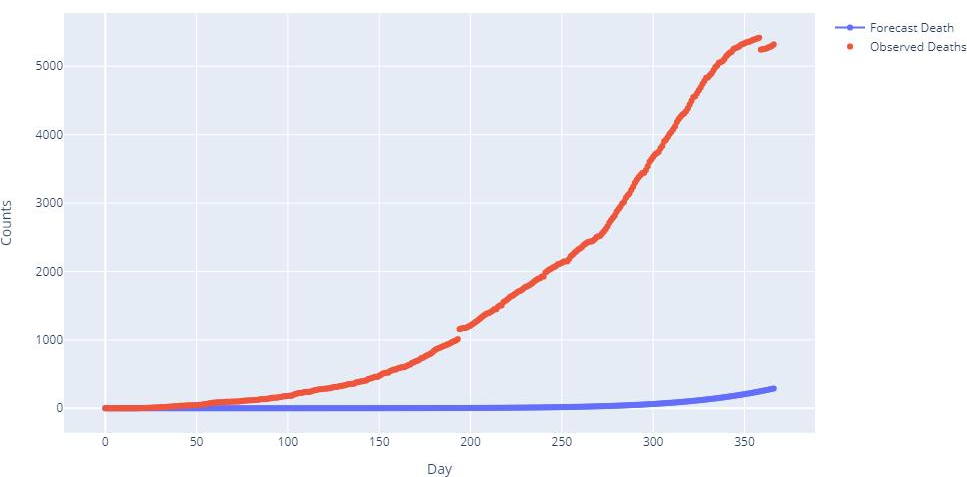
\includegraphics[width=0.5\linewidth]{figures/better_death.png}}
    \caption{疫情控制模型实际数据对比图}
\end{figure}

\clearpage
\subsection{结论}
观察在不同政策下疫情的发展趋势图,结合已有的在无疫苗情况下的图像,我们很容易得到以下结论:
\begin{enumerate}
    \item 疫苗对于防控疫情十分重要,体现在降低传染率和升高治愈率上。因此消灭疫情需要有效的疫苗和较高的接种率。
    \item 政府需要将疫苗接种和防止人员流动结合起来,既可以降低感染人数,使疫情无法大规模爆发,也可以保护人民的生命财产安全,增强社会稳定。
    \item 民众舆论会对政府政策造成一定影响,地区人群对于防疫措施的配合程度会进一步影响疫情发展,因此真实的疫情数据伴随着地区民众意愿有一定波动。
\end{enumerate}

\section{结论}
阿肯色州的疫情发展对我国的防疫措施有着一定的参考价值。疫情数据和预测结果均表明,
政府需要有强有力的措施来推行政策,且需要民众的积极配合。疫苗研发对于防止疫情爆发
有着决定性作用,同时可以最大程度保障人民生命安全。疫情期间需要对群众进行一定的医疗
知识宣传,尽可能增加疫苗的接种率,减少“疫苗谬论”,保证绝大多民众有疫苗接种意愿。美国
政府在疫情初期应对疫情不利,导致了后来多轮疫情的爆发;现阶段我国的疫情显著向好,应该
警惕各种疫情谣言,推进防疫政策,保证人群接种率,防止疫情的再度爆发。

\begin{thebibliography}{9}%宽度9
    \renewcommand\refname{}
    \bibitem[1]{英文论文}Przybylowski Adam,Stelmak Sandra,Suchanek Michal.
    \newblock Mobility Behaviour in View of the Impact of the COVID-19 Pandemic—Public Transport Users in Gdansk Case Study{}\allowbreak[J].
    \newblock Sustainability,2021,13(1).
    \bibitem[2]{英文论文2}Chang Serina,Pierson Emma,Koh Pang Wei,Gerardin Jaline,Redbird Beth,Grusky David,Leskovec Jure.
    \newblock Mobility network models of COVID-19 explain inequities and inform reopening {}\allowbreak[J].
    \newblock Nature,2020.
    \bibitem[3]{论文1}李瑞松,刘洪久.
    \newblock 基于传染病模型应用于中美两国应对COVID-19的对比研究 {}\allowbreak[J].
    \newblock 疾病预防控制通报,2021,36(02):1-5+21.
    \bibitem[4]{论文2}邹宇庭,郑晓练,缪旭晖,谭忠.
    \newblock SARS传播的数学原理及预测与控制{}\allowbreak[J].
    \newblock ⼯程数学学报,2003,20(07):29-34.
\end{thebibliography}

\clearpage
\begin{appendices}
    \section{完整可执行程序}
    \begin{minted}
        [
        numbers = left,
        linenos,
        numbersep=2pt,
        baselinestretch=1.2,
        fontsize=\footnotesize,
        breaklines,
        frame=single
        ]
        {python}
# python库导入
import os import sys
import matplotlib.pyplot as plt
import numpy as np
import pandas as pd
from scipy.integrate import odeint
import plotly.graph_objects as go
import plotly.io as pio
from lmfit import minimize, Parameters, Parameter, report_fit
pio.renderers.default = "notebook"
%matplotlib inline plt.style.use('ggplot')

# 读取数据,绘图的功能模块
from IPython.display import HTML
from ipywidgets.widgets import interact, IntSlider, FloatSlider, Layout, ToggleButton, ToggleButtons
style = {'description_width': '100px'}
slider_layout = Layout(width='99%')

# 图形处理有关
def ode_model(z, t, beta, sigma, gamma, mu): 
    """ Reference https://www.idmod.org/docs/hiv/model-seir.html """
    S, E, I, R, D = z
    N = S + E + I + R + D
    dSdt = -beta * S * I / N
    dEdt = beta * S * I / N - sigma * E
    dIdt = sigma * E - gamma * I - mu * I
    dRdt = gamma * I
    dDdt = mu * I
    return [dSdt, dEdt, dIdt, dRdt, dDdt]

# 微分方程传播模型求解
def ode_solver(t, initial_conditions, params):
    initE, initI, initR, initN, initD = initial_conditions
    beta, sigma, gamma, mu = params['beta'].value, params['sigma'].value, params['gamma'].value, params['mu'].value
    initS = initN - (initE + initI + initR + initD)
    resl = odeint(ode_model, [initS, initE, initI, initR, initD], t, args= (beta, sigma, gamma, mu))
    return resl

# 解常微分方程的函数
df1= pd.read_csv('covid_tracking.csv', sep=',') df_AR = df1.query('state=="AR"') # 阿肯色州
# df_AR.describe() df_temp = df_AR.iloc[::-1]
df_temp.reset_index(drop=True,inplace=True)
df_temp2= df_temp.loc[:, ['date', 'positive','recovered','death']] # df_temp2.tail()
values = {'death': 0,'recovered': 0} df_temp2.fillna(value=values,inplace=True)

# 全部初始化参数
initN = 2830000
initE = 10
initI = 20
initR = 0
initD = 0
sigma = 0.0010
gamma = 0.006
mu = 0.0012
R0 = 2
beta = 4
days = 340
params = Parameters()
params.add('beta', value=beta, min=0, max=10)
params.add('sigma', value=sigma, min=0, max=10)
params.add('gamma', value=gamma, min=0, max=10)
params.add('mu', value=mu, min=0, max=10)

# 演示效果动态调参
def main(initE, initI, initR, initD, initN, beta, sigma, gamma, mu, days, param_fitting):
    initial_conditions = [initE, initI, initR, initN, initD] params['beta'].value, params['sigma'].value,params['gamma'].value, params['mu'].value = [beta, sigma, gamma, mu] 
    tspan = np.arange(0, days, 1)
    sol = ode_solver(tspan, initial_conditions, params)
    S, E, I, R, D = sol[:, 0], sol[:, 1], sol[:, 2], sol[:, 3], sol[:, 4]

    # Create traces
    fig = go.Figure()
    fig1 = go.Figure()
    if not param_fitting:
        fig.add_trace(go.Scatter(x=tspan, y=S, mode='lines+markers', name= 'Susceptible'))
        fig.add_trace(go.Scatter(x=tspan, y=E, mode='lines+markers', name= 'Exposed'))
        fig.add_trace(go.Scatter(x=tspan, y=I, mode='lines+markers', name= 'Infected'))
        fig.add_trace(go.Scatter(x=tspan, y=R, mode='lines+markers',name=' Recovered'))
        fig.add_trace(go.Scatter(x=tspan, y=D, mode='lines+markers',name=' Death'))
        fig1.add_trace(go.Scatter(x=tspan, y=I, mode='lines+markers', name='Infected'))
        fig1.add_trace(go.Scatter(x=tspan, y=R, mode='lines+markers',name= 'Recovered'))
        fig1.add_trace(go.Scatter(x=tspan, y=D, mode='lines+markers',name= 'Death'))
    if param_fitting:
        fig.add_trace(go.Scatter(x=tspan, y=df_temp2.positive, mode='lines+markers',name='Infections Observed', line = dict(dash= 'dash')))
        fig.add_trace(go.Scatter(x=tspan, y=df_temp2.recovered, mode='lines+markers',name='Recovered Observed', line = dict(dash=' dash')))
        fig.add_trace(go.Scatter(x=tspan, y=df_temp2.death, mode='lines+markers',name='Deaths Observed', line = dict(dash='das h')))

    if days <= 30:
        step = 1
    elif days <= 90:
        step = 7
    else:
        step = 30

    # Edit the layout
    fig1.update_layout(title='SEIRD test',xaxis_title='Day',yaxis_title='Counts', title_x=0.5,width=1000, height=600)
    fig.update_layout(title='Simulation of SEIRD Model',xaxis_title='Day', yaxis_title='Counts', title_x=0.5,width=900, height=600)
    fig.update_xaxes(tickangle=-90, tickformat = None, tickmode='array', tickvals=np.arange(0, days + 1, step))
    if not os.path.exists("images"): os.mkdir("images")
        fig.write_image("images/seird_simulation.png")
        fig.show()

# 对应动态调参数图
interact(main,initE=IntSlider(min=0, max=100000, step=1, value=initE, description='initE', style=style, layout=slider_layout),
    initI=IntSlider(min=0, max=100000, step=10, value=initI, description='initI', style=style, layout=slider_layout),
    initR=IntSlider(min=0, max=100000, step=10, value=initR, description='initR', style=style, layout=slider_layout),
    initD=IntSlider(min=0, max=100000, step=10, value=initD, description='initD', style=style, layout=slider_layout),
    initN=IntSlider(min=0, max=1380000000, step=10000, value=initN, description='initN', style=style, layout=slider_layout),
    beta=FloatSlider(min=0, max=4, step=0.01, value=beta, description='Infection rate', style=style, layout=slider_layout),
    sigma=FloatSlider(min=0, max=4, step=0.01, value=sigma, description='Incubation rate', style=style, layout=slider_layout),
    gamma=FloatSlider(min=0, max=4, step=0.01, value=gamma, description='Recovery rate', style=style, layout=slider_layout),
    mu=FloatSlider(min=0, max=1, step=0.001, value=mu, description='Mortality rate', style=style, layout=slider_layout),
    days=IntSlider(min=0, max=600, step=7, value=days, description='Days', style=style, layout=slider_layout),
    param_fitting=ToggleButton(value=False, description='Fitting Mode', disabled=False, button_style='',
    tooltip='Click to show fewer plots', icon='check-circle'))
# 误差分析
def error(params, initial_conditions, tspan, data):
    sol = ode_solver(tspan, initial_conditions, params)
    return (sol[:, 2:5] - data).ravel()

# 历史数据拟合
initial_conditions = [initE, initI, initR, initN, initD] 
beta = 4
sigma = 0.0012
gamma = 0.006
mu = 0.0001
params['beta'].value = beta
params['sigma'].value = sigma
params['gamma'].value = gamma
params['mu'].value = mu
days = 340
tspan = np.arange(0, days, 1)
data = df_temp2.loc[0:(days-1), ['positive', 'recovered', 'death']].values

print(initial_conditions)
print(params)

# 输出拟合结果
# fit model and find predicted values
result = minimize(error, params, args=(initial_conditions, tspan, data), method='leastsq') 
report_fit(result)

# 根据历史数据生参数
final = data + result.residual.reshape(data.shape) 
temp_days = 120
fig = go.Figure()
fig.add_trace(go.Scatter(x=tspan, y=data[:, 0], mode='markers', name='Obse rved Infections', line = dict(dash='dot')))
fig.add_trace(go.Scatter(x=tspan, y=data[:, 1], mode='markers', name='Obse rved Recovered', line = dict(dash='dot')))
fig.add_trace(go.Scatter(x=tspan, y=data[:, 2], mode='markers', name='Obse rved Deaths', line = dict(dash='dot')))
fig.add_trace(go.Scatter(x=tspan, y=final[:, 0], mode='lines+markers', name='Fitted Infections'))
fig.add_trace(go.Scatter(x=tspan, y=final[:, 1], mode='lines+markers', name='Fitted Recovered'))
fig.add_trace(go.Scatter(x=tspan, y=final[:, 2], mode='lines+markers', name='Fitted Deaths'))
fig.update_layout(title='SEIRD: Observed vs Fitted',xaxis_title='Day', yaxis_title='Counts', title_x=0.5,width=1000, height=600)

    \end{minted}
\end{appendices}
\end{document}